\documentclass[a4paper,10pt, notitlepage]{report}
\usepackage[utf8]{inputenc}
\usepackage{natbib}
\usepackage{amssymb}
\usepackage{amsmath}
\usepackage[shortlabels]{enumitem}
% \usepackage[portuguese]{babel}
\usepackage{graphicx}
\usepackage{hyperref}
\usepackage{url}

\newcommand{\ev}{\mathbb{E}}
\newcommand{\var}{\operatorname{Var}}


% Title Page
\title{Assignment 1: Algorithms Galore! \\\vspace{2mm}
       \normalsize Chosen algorithm: Rejection Sampling
}
\author{Computational Statistics \\ Student: Lucas Machado Moschen \\ Instructor: Luiz Max de Carvalho}

\begin{document}
\maketitle

\textbf{Hand-in date: 22/11/2021.}

\section*{General guidance}
\begin{itemize}
 \item State and prove all non-trivial mathematical results necessary to substantiate your arguments;
 \item Do not forget to add appropriate scholarly references~\textit{at the end} of the document;
 \item Mathematical expressions also receive punctuation;
 \item Please hand in a single PDF file as your final main document.
 
 Code appendices are welcome,~\textit{in addition} to the main PDF document.
 \end{itemize}

\newpage

\section*{Background}

By now we have seen quite a few methods for computing integrals~\textit{via} Monte Carlo.
Each method has its own advantages and drawbacks.
It is important that we understand these properties in order to apply the methods effectively. 
In this assignment we will continue studying the problem of computing the average distance between two points on a disk, this time from the perspective of method comparison.
That is to say that in this assignment you will experience the microcosm of comparing several methods for solving a problem for which we happen to know the right answer in closed-form.

Recall that we want to compute 
 \begin{align*}
  I &= \frac{1}{\pi^2 R^4}\int_{0}^{R}\int_{0}^{R}\int_{0}^{2\pi}\int_{0}^{2\pi}\sqrt{r_1^2 + r_2^2 - 2r_1r_2\cos\phi(\theta_1, \theta_2)}r_1r_2\,d\theta_1\,d\theta_2\,dr_1\,dr_2,\\
  &= \frac{128}{45\pi}R,
 \end{align*}
 where $\phi(\theta_1, \theta_2)$ is the central angle between $r_1$ and $r_2$.
 
Here we will do something a bit risky: we will compare a few methods to compute $I$ using a bunch of different methods without knowing in advance which will work best or if there are going to be any differences at all.
Welcome to Science!


\section*{Methods}

Here we will list a selection of methods that will be randomly assigned to each student, along with some questions that need to be answered for that particular method.
\begin{itemize}
 \item \textbf{Rejection sampling}
  \begin{itemize}
  \item Justify your choice of proposal distribution and show that it conforms to the necessary conditions for the algorithm to work; in particular, try to find a proposal that gives the highest acceptance probability.
 \end{itemize}
  \item \textbf{Importance sampling}
 \begin{itemize}
  \item Justify your choice of proposal based on the variance of the resulting estimator.
 \end{itemize}
  \item \textbf{Gibbs sampling}
 \begin{itemize}
  \item Write your full conditionals out and show that they adhere to the Hammersley-Clifford condition.
 \end{itemize}
  \item \textbf{Metropolis-Hastings}
 \begin{itemize}
  \item Justify your choice of proposal; test different ones if you need to.
 \end{itemize}
 \item \textbf{Static Hamiltonian Monte Carlo}
 \begin{itemize}
  \item Comment on the choice of step size ($\varepsilon$) and integration time ($\tau$).
 \end{itemize}
\end{itemize}


\section*{Questions}

\begin{enumerate}
 \item You have been (randomly) assigned a method from the previous section.
 Represent $I$ as $\int_{\mathcal{X}} \phi(x)\pi(x)\,dx$ and justify your choice of $\phi$, $\pi$ and $\mathcal{X}$.
 Recall that these choices are arbitrary up to a point, but they might lead to wildly different empirical performances~\textbf{and} theoretical properties for estimators of $I$.
 \textbf{Justify} your choices in light of the method you have been given to work with.
 Choose wisely and be rigorous in your justifications.
 \item Again, starting from the eventual samples you will obtain with your meth-od, construct a non-empty\footnote{This is a joke. It means you should come up with at least one estimator. But you might, and are even encouraged to, entertain more than one estimator.} family of estimators of $I$ and discuss whether it is (strongly) consistent and whether a central limit theorem can be established.
 \item Detail a suite of diagnostics that might be employed in your application to detect convergence or performance problems.
 Extra points for those who design algorithms that exploit the structure of this particular integration problem. 
 \item For each $R \in \{0.01, 0.1, 1, 10, 100, 1000, 10000\}$, perform $M=500$ runs from your simulation method and compute: (i) variance (ii) bias (iii) standard deviation of the mean (MCSE).
 \item Can you identify one key quantity missing from the previous item?
 \textit{Hint:} it bears relevance to the real world application of any computational method.
\end{enumerate}

\textbf{Warning:} the questions in this assignment might seem deceptively simple; do not be fooled. I expect a lot of effort from you in making your method work the best it can. This entails loads of failed derivations and experiments, which you are encouraged to report in order to document the discovery process.
Also, feel free to include answers to questions that have not been asked, if you feel they are relevant. 
Make loads of figures and tables and let your scientific imagination run wild! 
Good luck! 

\newpage

\section*{Rejection Sampling}

To obtain a sample from distribution $\pi$, the ideia of Rejection Sampling
method is to sample from a distribution $q$ and reject some of the samples to
correct the distribution of the sampling. If for all values of $x \in
\mathcal{X}$, $\pi(x) \le Mq(x)$, the acceptance probability is 
$$
\alpha = \frac{\pi(x)}{Mq(x)}.
$$
The number of necessary samples until acceptance has Geometric Distribution
with parameter $1/M$ \cite[p. 51]{robert2004monte}. To calculate an
approximation for the integral $I$ through this method, we must define 
a target distribution $\pi$ up to a normalizing constant and $q$ such that
$\pi/q$ be bounded by $M$ in $\mathcal{X}$. The presentation is in the order 
of the discovery process. 

\section*{A simple first derivation}

The simplest method is to define $\pi(x) \propto 1$ para $x \in [0,R]^2
\times [0,2\pi]^2$. Since we have a method for sampling from $\pi$, we can 
define $q = \pi$ and $M=1$. Our Monte Carlo estimator is therefore 
$$
\hat{I}_1 = \frac{4}{mR^2}\sum_{i=1}^m \sqrt{\left(r_1^{(i)}\right)^2 + \left(r_2^{(i)}\right)^2 - 2r_1^{(i)}r_2^{(i)}\cos\left(\theta_2^{(i)} - \theta_1^{(i)}\right)}r_1^{(i)}r_2^{(i)},
$$
where $x^{(i)} = \left(r_1^{(i)}, r_2^{(i)}, \theta_1^{(i)},
\theta_2^{(i)}\right)$ is a sample from $\pi(x)$. This estimator can be
simplified with $\pi(x) \propto 1$ for $x \in [0,1]^4$ with
$$
\hat{I}_2 = \frac{4R}{m}\sum_{i=1}^m \sqrt{\left(x_1^{(i)}\right)^2 + \left(x_2^{(i)}\right)^2 - 2x_1^{(i)}x_2^{(i)}\cos\left(2\pi\left(x_4^{(i)} - x_3^{(i)}\right)\right)}x_1^{(i)}x_2^{(i)},
$$
decreasing the number of required multiplications. Another advantage of
$\hat{I}_2$ over $\hat{I}_1$ is that the samples can be reused for different
values of $R$. Both $\hat{I}_1$ and $\hat{I}_2$ have the advantage of
enabling the calculation of their variance. The second moment of each term of $\hat{I}_1$ is
\begin{align*}
    &\frac{1}{4\pi^2 R^2}\int_{0}^{R}\int_{0}^{R}\int_{0}^{2\pi}\int_{0}^{2\pi}r_1^4r_2^2 + r_2^4r_1^2 - 2r_1^3r_2^3\cos(\theta_2 - \theta_1) \\
    &= \frac{1}{4\pi^2 R^2}\frac{8\pi^2 R^8}{15} = \frac{2R^6}{15}
\end{align*}
and the first moment is
\begin{equation}
    \label{eq:first-moment-term-I1}
    \begin{split}
        &\frac{1}{4\pi^2 R^2}\int_{0}^{R}\int_{0}^{R}\int_{0}^{2\pi}\int_{0}^{2\pi}\sqrt{r_1^2 + r_2^2 - 2r_1r_2\cos(\theta_2 - \theta_1)}r_1r_2 \\
        &= \frac{R^2}{4} I = \frac{32R^3}{45\pi}.     
    \end{split}
\end{equation}
Therefore the variance is 
\begin{equation*}
    \begin{split}
        \var[\hat{I}_1] &= \frac{4^2}{mR^4}\left(\frac{2R^6}{15} - \frac{1024R^6}{45^2\pi^2}\right) \\
        &= \frac{1}{m}\left(\frac{32}{15} - \frac{2^{14}}{45^2\pi^2}\right)R^2 \approx \frac{1.31}{m}R^2. 
    \end{split}    
\end{equation*}

Moreover, this estimator is unbiased by relation
\eqref{eq:first-moment-term-I1}. Similar calculations for $\hat{I}_2$ indicate
the same variance, since only linear transformations are made. By the Strong
law of large numbers, with the $\hat{I}_1$ and $\hat{I}_2$ converges to the
integral $I$  with probability 1. The central limit theorem give bounds for
this convergence, stating that 
$$
\sqrt{m}(\hat{I}_1 - I) \overset{d}{\to} \operatorname{Normal}(0, 1.31R^2). 
$$
This proposal also gives the highest acceptance probability, as required. 

\section*{Regular polygon circumscribed around a circle}

When trying to find an approximation for $\pi$, the ratio of the circumference
of a circle to its diameter, Archimedes noticed that taking the mean between
the perimeters of a $n$-regular circumscribed polygon and a $n$-regular
inscribed polygon, the result would converge to the circumference of the
circle. Here the ideia is to sample from the circumscribed polygon with $n$
sides and use the rejection sampling to obtain the distribution $\pi(x)$. 

First, we reparametrize integral $I$ in Cartesian coordinates 
$$
\int_{\mathcal{X}} \sqrt{(p_x - q_x)^2 + (p_y - q_y)^2} \pi(x) \, dp_x\, dp_y\, dq_x\, dqy, 
$$
where $\mathcal{X}$ is the circle of radius $R$ and $\pi(x)$ is the uniform
distribution over $\mathcal{X}$. 

We define $q_n$ to be the uniform distribution over the circumscribed polygon
of $n$ sides and we must develop a method to sample from $q$. First of all, we
break the circle in $n$ equal pieces as presented in Figure \ref{fig:figure1}.
A circumscribed polygon has its sides tangent to the circle at the midpoints
between the red ones. Figure \ref{fig:figure2} presents the tangent points in
blue. 

\begin{figure}[htpb]
    \centering
    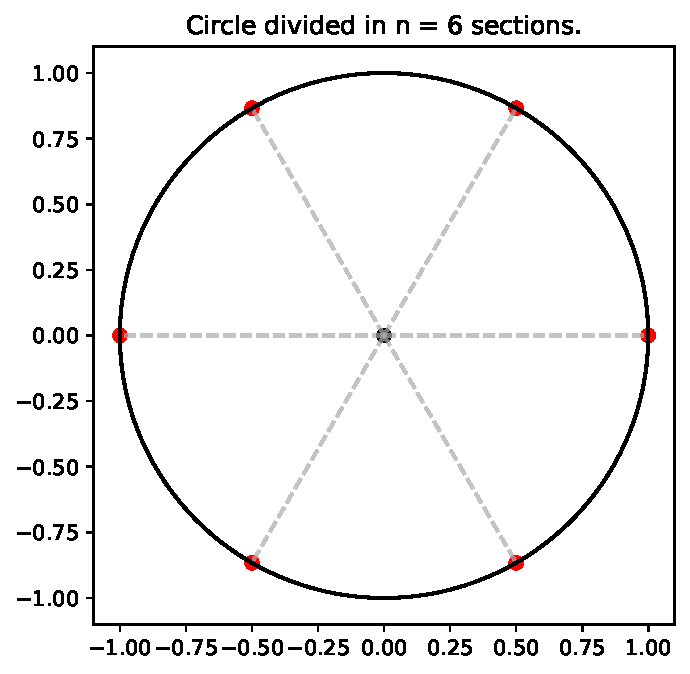
\includegraphics[width=6cm]{images/figure1.pdf}
    \caption{\label{fig:figure1}Circle divided in $n=6$ sections delimited by
    the red points and the grey lines.}
\end{figure}

Let $(x_m, y_m)$ be a midpoint between two red points $(x_1, y_1)$ and
$(x_2, y_2)$. The tangent line over the circle passing por that point has the
following expression
$$
y = -\frac{x_m}{y_m}(x - x_m) + y_m,
$$
which is derived with implicit differentiation for $x^2 + y^2 = R^2$.
Moreover, the line passing through the center of the circle and the red points
is given by
$$
y = \frac{y_1}{x_1}x.
$$

\begin{figure}[htpb]
    \centering
    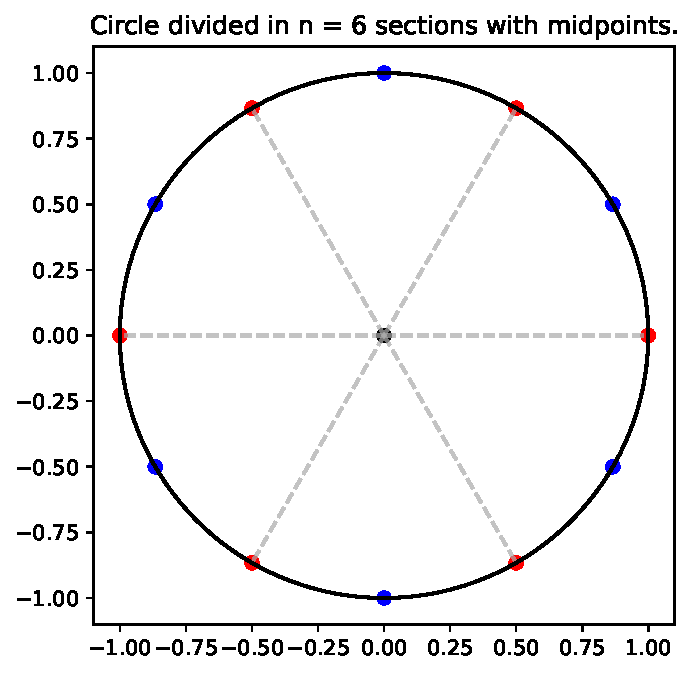
\includegraphics[width=6cm]{images/figure2.pdf}
    \caption{\label{fig:figure2}Circle divided in $n=6$ sections and midpoints
    in blue.}
\end{figure}

They cross at the point
$$
-\frac{x_m}{y_m}(x - x_m) + y_m = \frac{y_1}{x_1}x \implies x = \dfrac{\frac{x_m^2}{y_m} + y_m}{\frac{x_m}{y_m} + \frac{y_1}{x_1}}, 
y = \frac{y_1}{x_1}x.
$$
After extending the segments splitting the circle, we can build the polygon
as Figure \ref{fig:figure3} presents in green. Figure \ref{fig:figure4} shows
the same construction for different values of $n$. Notice that when $n=12$,
the approximations already is quite good. 

\begin{figure}[htpb]
    \centering
    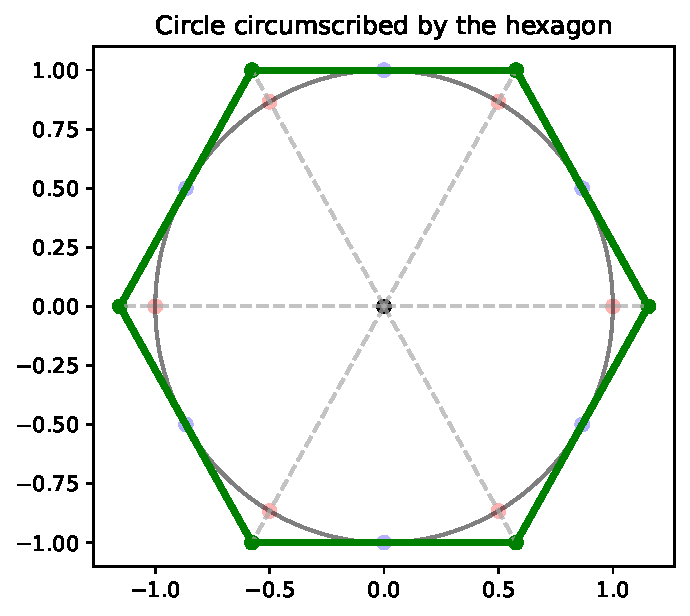
\includegraphics[width=6cm]{images/figure3.pdf}
    \caption{\label{fig:figure3}Hexagon circumscribing the circle.}
\end{figure}

\begin{figure}[htpb]
    \centering
    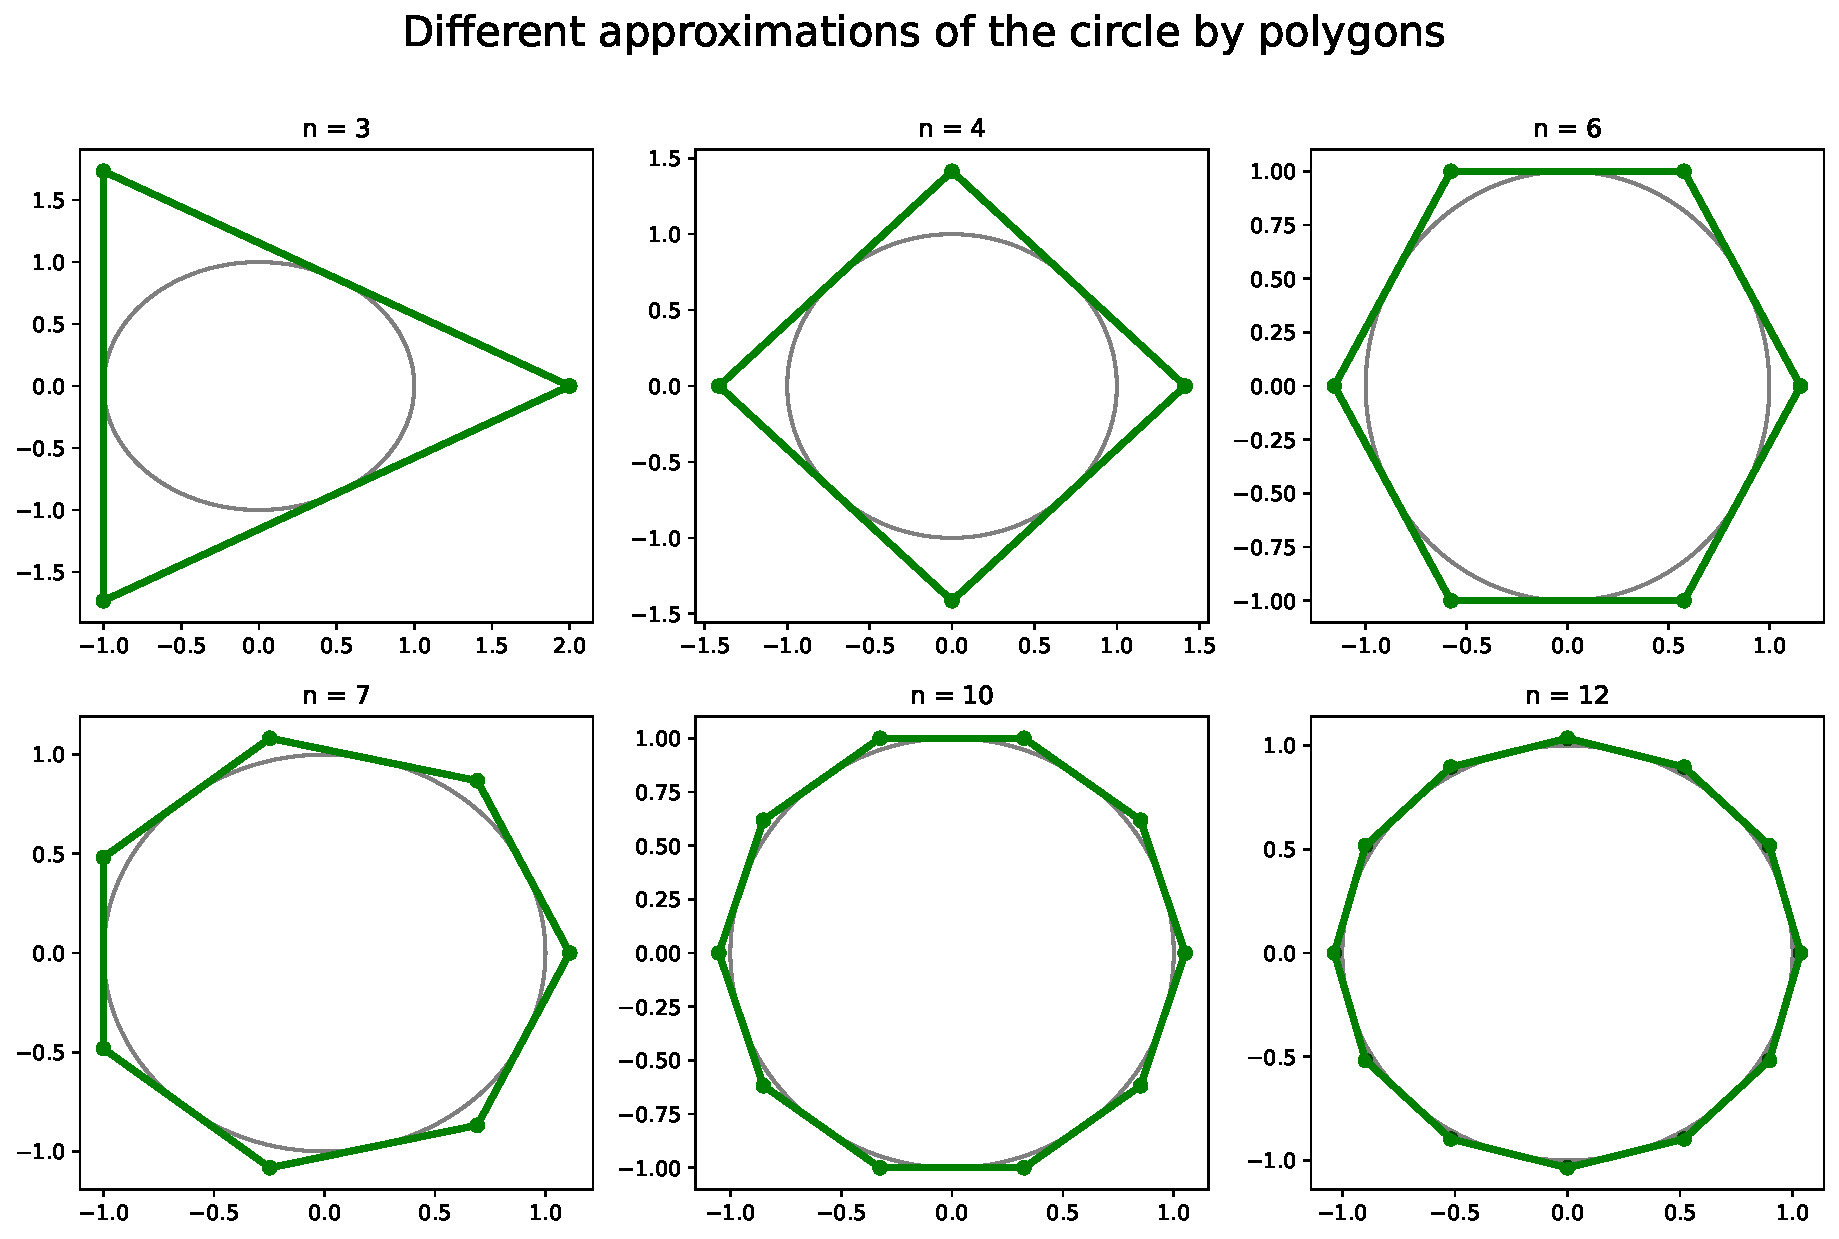
\includegraphics[width=12cm]{images/figure4.pdf}
    \caption{\label{fig:figure4}Different polygons approximating the circle.}
\end{figure}

Now that we are able to build an arbitrarily polygon with $n$ sides, we need
to know how to sample uniformly from it. Notice that the region delimited
by the circle is included in the region delimited by the polygon. 
Since we separated the polygon in $n$ sections, we perform the following algorithm:

\begin{enumerate}[(i)]
    \item Draw $i \sim \operatorname{Unif}\{1, \dots, n\}$ and pick the
    corresponding section delimited by the points $(0,0), (x_i, y_i),
    (x_{i+1}, y_{i+1})$ in the polygon. If $i=n$, we change $i+1$ for $1$;
    \item Draw uniformly from the corresponding triangle.
\end{enumerate}

We have to specify how to sample inside a specific triangle delimited for
three points. Fortunately, this is not a hard thing. Let $u_1, u_2 \sim
\operatorname{Unif}[0,1]$. The sum vector
$$
v= u_1(x_i, y_i) + u_2(x_{i+1}, y_{i+1})
$$
is contained in the parallelogram formed by twice the triangle. Figure
\ref{fig:figure5} shows this relation for 10000 samples. To chop the part we
do not want to, we have to reflect each point outside the triangle to inside
the triangle. If $u_1 + u_2 \le 1$, the point $v$ is inside the triangle.
Otherwise, denote $v_1 = 1 - u_1 \operatorname{Unif}[0,1]$ and $v_2 = 1 - u_2
\operatorname{Unif}[0,1]$, and we will have $v_1 + v_2 = 2 - (u_1 + u_2) \le
1$. In that sense, we are mapping each point outsize to one inside. Therefore,
the uniformity is kept. Figure \ref{fig:figure6} presents the result of the
algorithm. Therefore, we know how to sample from $q_n$. 

\begin{figure}[htb]
    \centering
    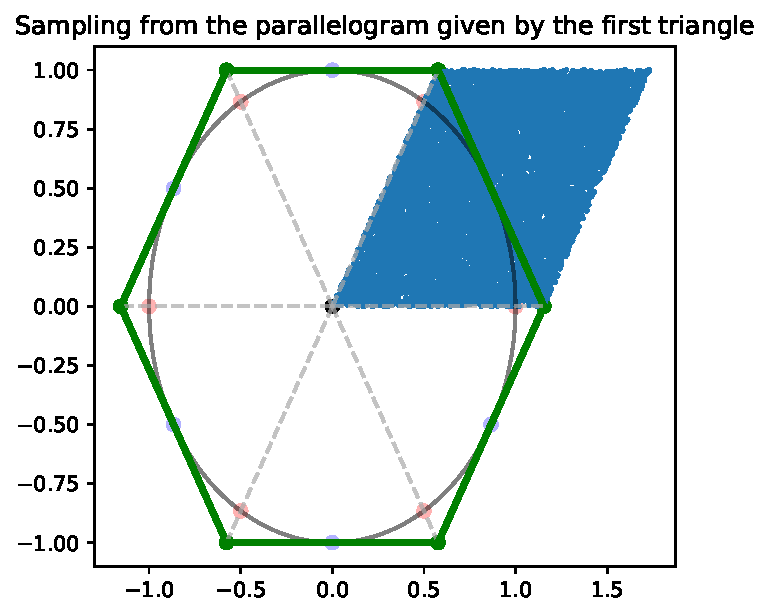
\includegraphics[width=6cm]{images/figure5.pdf}
    \caption{\label{fig:figure5}Different polygons approximating the circle.}
\end{figure}

\begin{figure}[htb]
    \centering
    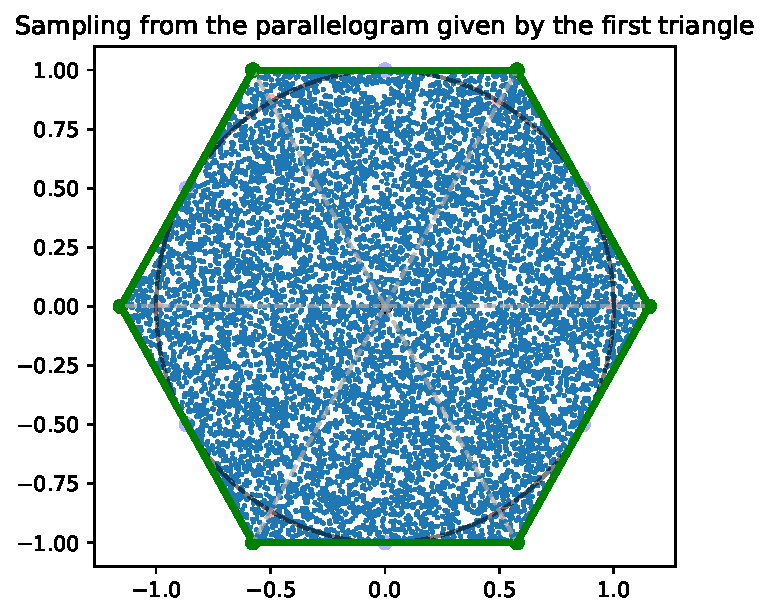
\includegraphics[width=6cm]{images/figure6.pdf}
    \caption{\label{fig:figure6}Sampling uniformly in the hexagon.}
\end{figure}

We also know to calculate the area of the circumscribing polygon of $n$-sides
by the formula \cite{efunda2021formula}
$$
A = nR^2\tan\left(\frac{\pi}{n}\right).
$$
Therefore, 
$$
\pi(x) = \frac{1}{\pi^2R^4}, q_n(x) = \frac{1}{n^2R^4\tan^2(\frac{\pi}{n}} \implies \frac{\pi(x)}{q(x)} =
\frac{(n\sin(\pi/n))^2}{\cos^2(\pi/n)\pi^2}
$$
From that, for each $n$ we calculate
$$M_n = \frac{(n\sin(\pi/n))^2}{\cos^2(\pi/n)\pi^2},$$
the average number of samples until acceptance. Observe that 
$$
\lim_{n\to \infty} M_n = \frac{1}{\pi^2} \left(\lim_{x \to 0^+} \frac{\sin(x\pi)}{x}\right)^2
= \left(\lim_{y \to 0^+} \frac{\sin(y)}{y}\right)^2 = 1,
$$
as expected. Figure \ref{fig:figure7} show several values for $M_n$ for
different values of $n$. 

\begin{figure}[htpb]
    \centering
    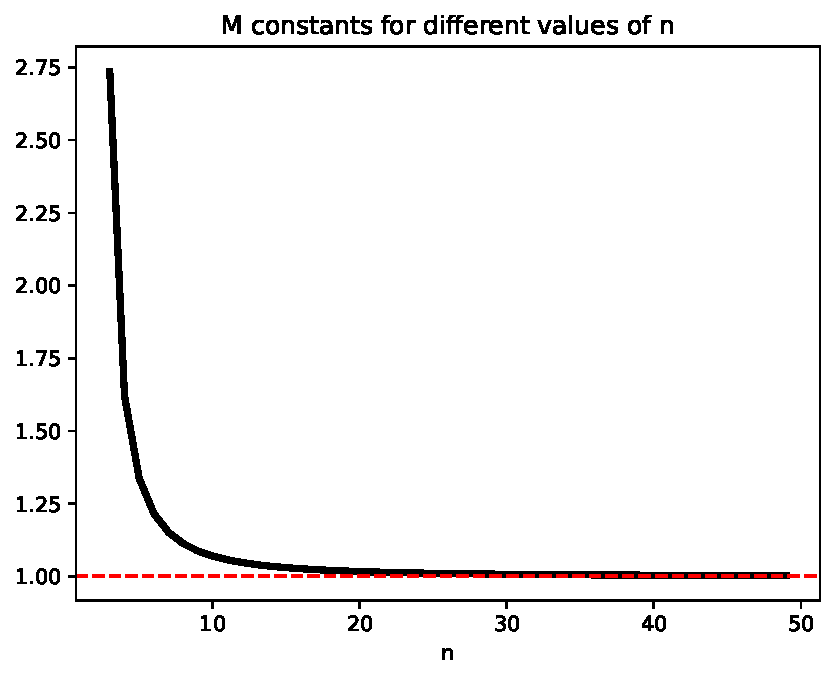
\includegraphics[width=7cm]{images/figure7.pdf}
    \caption{\label{fig:figure7}The red line delimits the limit value.}
\end{figure}

After sampling from $q_n$ distribution, to obtain $\pi$ through Rejection
sampling, we must reject samples $(x^{(i)}, y^{(i)})$ such that 
$$(x^{(i)})^2 + (y^{(i)})^2 > R^2.$$ This summarizes in a simple algorithm: 

\begin{enumerate}[(i)]
    \item Fix the number of sides $n$ and number of samples $m$;
    \item Construct the polygon of $n$ sides; 
    \item Repeat $m$ times: 
    \begin{itemize}
        \item Sample $i \sim \operatorname{Unif}\{1, \dots, n\}$. Let $T$ be the
        triangle delimited by the points $(0,0), (x_i, y_i), (x_{i+1}, y_{i+1})$.
        If $i=n$, substitute $i+1$ for $0$; 
        \item Sample $v_1, v_2 \sim \operatorname{Unif}[0,1]$. If $v_1 + v_2 >
        1$, let $u_1 = 1 - v_1$ and $u_2 = 1 - v_2$. Otherwise let $u_1 = v_1$
        and $u_2 = v_2$; 
        \item If $||u_1(x_i, y_i) + u_2(x_{i+1}, y_{i+1})||^2 > R^2$, ignore
        this step and repeat it. Otherwise save the sample 
        $$p = u_1(x_i, y_i) + u_2(x_{i+1}, y_{i+1}).$$
    \end{itemize} 
\end{enumerate}

With the sample from $p^{(i)}, q^{(i)} \sim \pi(x)$ built by Rejection Sampling, we
introduce 
$$
\hat{I}_3 = \frac{1}{m} \sum_{i=1}^m ||q^{(i)} - p^{(i)}||. 
$$
This is an unbiased estimator, consistent with asymptotic distribution 
similar to $\hat{I}_1$. The disadvantage of $\hat{I}_3$ is the wasted samples,
but it introduces a class of estimators that depend on the number of the sides
of a polygon. 

\section*{Diagnosis}

\section*{Experiments}

Evaluate variance, bias, MCSE, and $\hat{R}$. 

\bibliographystyle{apalike}
\bibliography{../stat_comp}

\end{document}          
